\label{chap:dataset_creation}

En este capítulo contaremos el diseño del proceso de recolección, selección y anotación de datos. Por lo marcado en anteriores secciones, consideramos interesante el problema de hacer una detección de lenguaje discriminatorio bajo un contexto. Es decir, no es lo mismo considerar el mensaje ``sos un hombre'' en solitario que si ese mismo mensaje está dirigido hacia una mujer trans.

Nos abocamos a la decisión de crear un dataset que no sólo contenga un mensaje/comentario, sino que provea un contexto en el cual se da este mensaje. Un ámbito natural para esta tarea son las notas periodísticas, donde disponemos de una nota y comentarios realizados sobre esta. Un ejemplo puede verse .

Muchos sitios de noticias disponen de sistemas embebidos de comentarios, pero vista la dificultad para la recolección a la vez que los limitados datos provistos por estos sitios nos llevaron a buscar otro medio: Twitter. Twitter provee una sencilla API para descargar datos, a la vez

Algo a tener en cuenta es que este tipo de datos tiene una naturaleza particular, ya que las agresiones discriminatorias son usualmente a personajes públicos o colectivos de personas, y se dan de manera indirecta (a través del comentario en la noticia) y no directa (es decir, como respuesta al usuario de Twitter ofendido)

\section{Trabajos previos}
\label{sec:dataset_previous}

Pocos trabajos incorporan algún tipo de contexto a los comentarios del usuario para estas tareas. \citet{gao-huang-2017-detecting} construyó un dataset de lenguaje discriminatorio sobre 1518 comentarios del sitio de Fox News. A los anotadores les fue presentado tanto el comentario como la noticia a la hora de realizar el etiquetado. Sobre este dataset, efectuó experimentos de clasificación usando modelos lineales (regresiones logísticas) y modelos neuronales. En estos experimentos observó que un clasificador (tanto lineal como neuronal) mejora su performance al consumir el título de la noticia, dando indicios de que se puede aprovechar el contexto para mejorar la detección de este fenómeno. Sin embargo, como marca \citet{pavlopoulos2020toxicity} este trabajo cuenta con algunos problemas: en primer lugar, el tamaño del dataset es pequeño, y está extraído de sólo 10 noticias, lo cual limita los posibles contextos. A su vez, la anotación fue realizada mayormente por un único anotador, lo cual hace poco confiables las etiquetas. Luego, algunos detalles menores debieran ser analizados con mayor detalle, como por ejemplo la utilización de los nombres de usuarios como features predictivas.

\citet{mubarak-etal-2017-abusive} construyó un dataset en árabe sobre comentarios con contenido abusivo del portal Al Jazeera. Sin embargo, este daaset tiene un problema: los comentarios son sólo presentados a los anotadores sobre noticias, ignorando todo el thread de la conversación. Esto hace que el contexto sea parcial.


Paralelamente a nuestro trabajo, \citet{pavlopoulos2020toxicity} analiza el impacto de agregar contexto a la tarea de detección de toxicidad. En particular, plantea dos preguntas

\begin{itemize}
    \item ¿Qué tanto afecta el contexto a la toxicidad percibida por humanos en conversaciones online?
    \item ¿Puede el contexto ayudar a mejorar la performance de clasificadores de toxicidad en comentarios?
\end{itemize}

Para responder estas preguntas, los autores construyeron dos datasets en base a Wikipedia Talk Pages\cite{hua-etal-2018-wikiconv}, un dataset de discusiones del sitio de Wikipedia. En primer lugar, armaron un dataset de 250 comentarios anotados por dos grupos disjuntos de anotadores: uno de los grupos anotó los comentarios de manera contextualizada, viendo tanto el comentario en cuestión como el título de la discusión; el otro grupo sólo vio el comentario a anotar sin contexto alguno. En dicho experimento observaron que los anotadores contextualizados percibieron 6.4\% de comentarios tóxicos versus un 4.4\% de quienes anotaron sin contexto, una diferencia significativa aplicando un test Mann-Whitney. Desagregando estos resultados, observaron que 13 de los 250 comentarios (5.2\%) tuvieron diferencias de anotación entre los dos grupos, con 9 (3.6\%) comentarios donde aumentó la toxicidad percibida y 4 comentarios donde bajó la toxicidad al ser agregado el contexto.

Para responder la segunda pregunta, anotaron un dataset de 20k comentarios, 10k anotados por un grupo que etiquetó viendo el contexto y otros 10k que no lo vio. Entre todos los comentarios del dataset original de Wikipedia Talk Pages, eligieron aquellos con profundidad entre 2 (respuestas directas) a 5, y con entre 10 y 400 caracteres de largo. Luego, entrenaron varios clasificadores usando este dataset y allí pudieron observar que el contexto no pareciera mejorar la performance. En el próximo capítulo nos extenderemos sobre las técnicas utilizadas por este trabajo.

\citet{xenos-2021-context} continúa el trabajo de \citet{pavlopoulos2020toxicity} desagregando el resultado de la segunda pregunta. Puntualmente, y observando que sólo un porcentaje pequeño de los comentarios parecen ser incididos por el contexto en el trabajo previo, construyen una nueva tarea: estimación de sensibilidad al contexto. Para ello, toman el dataset de Civil Comments\cite{borkan2019civil}, y reanotan un subconjunto de este dataset usando información de contexto a través de crowdsourcing. Las etiquetas de este dataset son de toxicidad en un estilo similar a una regresión ordinal, entendiendo las categorías no tóxico, incierto, tóxico, y muy tóxico. Ahora, teniendo las anotaciones originales del dataset (que fueron hechas sin contexto) y las nuevas anotaciones, pueden definir para cada comentario una sensibilidad al contexto, dada por

\begin{equation}
    \delta(p) = s^{oc}(p) - s^{ic}(p)
\end{equation}

donde $s^{oc}$ es la fracción de anotadores sin contexto que marcaron toxicidad, y $s^{ic}$ los que no tienen contexto.

\citet{sheth2021defining} señala algunas oportunidades para incorporar fuentes de información más ricas a la tarea de detección de toxicidad, como el historial de interacción entre los usuarios, el contexto social y otras bases de conocimiento externas.

\citet{wiegand2021implicitly} menciona formas implícitas de abuso, mucho más complejas que las basadas solamente en palabras ofensivas. Por ejemplo, deshumanizaciones (``los judíos son una plaga que merece ser eliminada''), llamadas a la acción (``hay que tirar una bomba en ese país''), acusaciones (``los chinos inventaron el coronavirus''), entre otros tipos sutiles de comportamiento tóxico. Así mismo, menciona que la mayoría de los datasets no consiguen capturar estos fenómenos debido a la forma de recolección usualmente basada en keywords.

\section{Recolección de noticias y comentarios}

\begin{table*}[t]
    \centering
    \begin{tabular}{ c|c|c }
        coronavirus  &  encierro          & síntomas \\
        covid        &  fase              & dengue   \\
        cuarentena   &  infectados        & aedes    \\
        normalidad   &  Wuhan             & mosquito \\
        aislamiento  &  distanciamiento   & cacharro \\
        padecimiento &  fiebre            &          \\
    \end{tabular}
    \caption{Words used to retrieve COVID-19 and Dengue related articles.\label{tab:article_words}}
\end{table*}


%%
%%
%%
%% https://docs.google.com/drawings/d/1IcBITgNJN-tehmvnZqcSF9cUuWIpNKJg6yHI5yjNF9c/edit
%%
%%

\begin{figure}
    \centering
    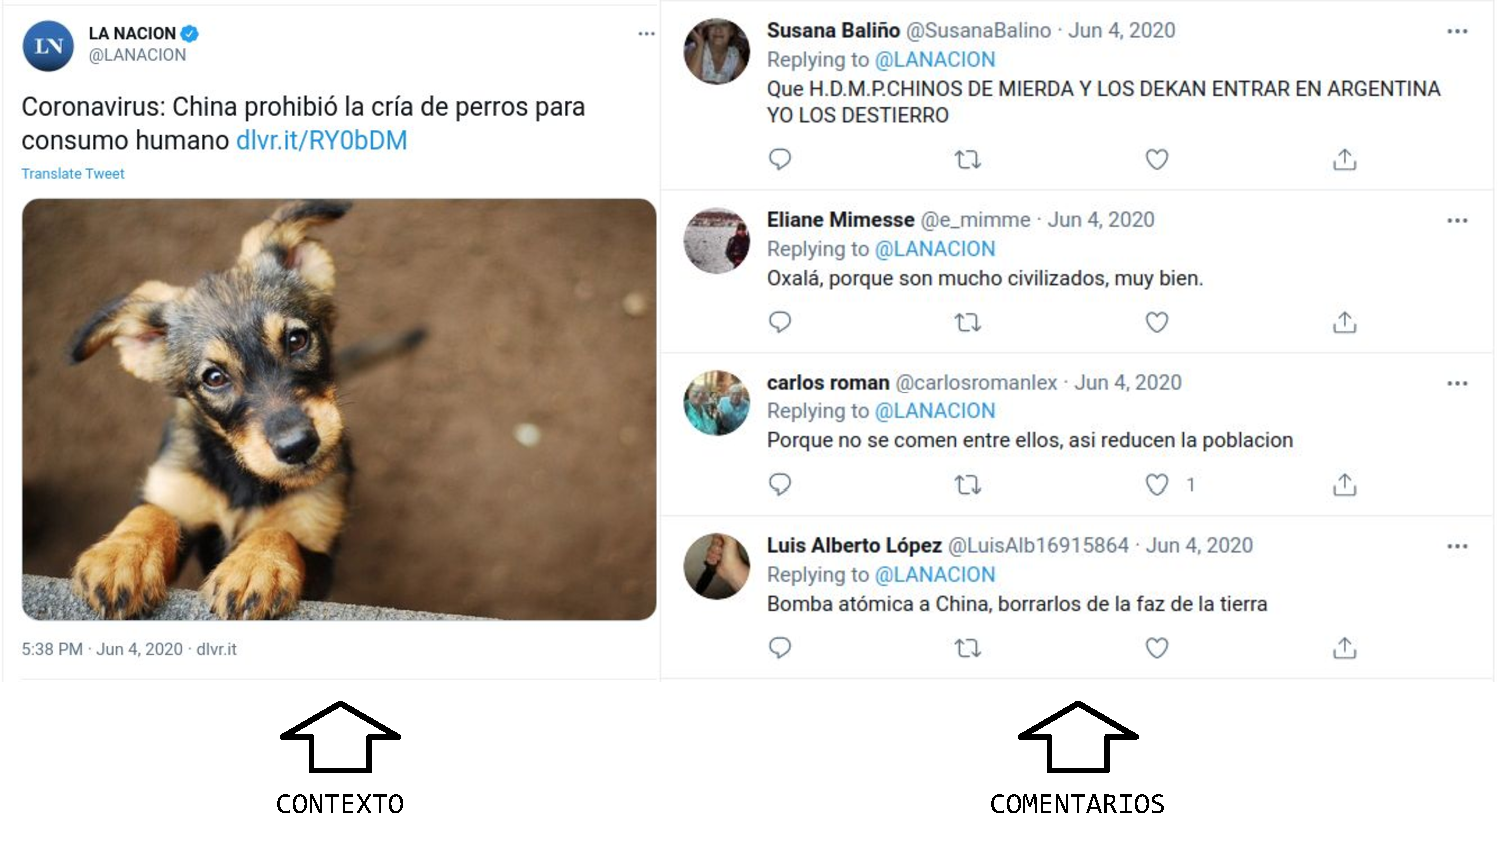
\includegraphics[width=\textwidth]{img/idea_dataset.pdf}
    \caption{Muestra de la recolección de datos}
    \label{fig:idea_dataset}
\end{figure}




Usamos la API de Twitter Stream mencionando cualquiera de estas cuentas. \todo{Explicar el proceso más detalladamente} Para cualquier tweet de uno de estos medios, reconstruimos la conversación. Para el propósito de este trabajo, solo estamos interesados en el primer nivel de respuestas al tweet original \footnote{Usamos una versión antigua de la API. La versión 2.0 parece facilitar la recopilación de conversaciones}. También eliminamos las URLs de los artículos de los enlaces.


Si bien consideramos otros medios (en particular, los ``periódicos'' electrónicos de derecha) decidimos apostar por medios más tradicionales con apoyo escrito: Clarín (@clarincom), La Nación (@LANACION), Infobae (@infobae), Perfil. (@perfilcom), Crónica (@cronicacom). Como el proceso de anotación iba a ser realizado por anotadores locales, decidimos no recopilar ningún dato de otros países de habla hispana.


El foco se hizo en artículos relacionados con COVID-19. Para ello, seleccionamos artículos buscando una cantidad de palabras en su cuerpo, por lo que seleccionamos específicamente artículos relacionados con COVID-19. La tabla \ref{tab: article_words} contiene las palabras utilizadas para recuperar estos artículos. También estábamos interesados en la pandemia del dengue; sin embargo, solo se recuperó un número muy pequeño de artículos.

La figura \ref{fig:idea_dataset} ilustra lo recolectado: en este caso, un tweet de un medio periodístico y todos los comentarios realizados sobre éste. En el caso de Twitter, los comentarios son respuestas al tweet original.


\subsection{Diarios elegidos}

Para esta tarea, elegimos 5 diarios:

\begin{itemize}
    \item Clarín
    \item La Nación
    \item Infobae
    \item Perfil
    \item Crónica
\end{itemize}

Estos diarios son los mayores generadores de contenido. Consideramos otros medios, pero nos atuvimos a medios formales tradicionales y con soporte escrito.

En un principio consideramos la posibilidad de anotar tweets de digiarios de otros países, pero teniendo en cuenta que esta tarea depende fuertemente de la jerga y de las variaciones dialectales de cada país decidimos realizar sólo anotación de estos diarios. A su vez, observamos que la mayoría de los comentarios son de la variedad dialectal rioplatense


\subsection{Datos recolectados}

\begin{table}[t]
    \centering
    \begin{tabular}{c|c|c}
    Medio      & \#Artículos recolectados & \#Comentarios \\
    \hline
    @infobae   &  45652   &  822462 \\
    @clarincom &  29050   &  672401 \\
    @perfilcom &  8764    &  61203  \\
    @LANACION  &  16040   &  506091 \\
    @cronica   &  17250   &  70872 \\
    \hline
    Total      & 116756  & 2133029 \\
    \end{tabular}
    \caption{Artículos recoletados por medio}
    \label{tab:articulos_recoletados_por_medio}
\end{table}


En la tabla \ref{tab:articulos_recoletados_por_medio} damos los números de los artículos recolectados por cada medio, luego de aplicado . Si bien recolectamos más artículos de otros medios, no son enumerados. Infobae es el medio que más producción de artículos genera, y también será finalmente sobre el que más comentarios etiquetemos.

La figura \ref{fig:fecha_articulos_por_medio_todas} muestra la distribución temporal de los artículos, sin aplicar ningún filtro por palabras, mientras que \ref{fig:fecha_articulos_por_medio_covid} muestra aquellas relacionadas al COVID-19 utilizando el filtro de palabras listado en la tabla \ref{tab:article_words}. Podemos observar dos caídas. Hay un pequeño pozo en mayo 2020 que se debió a la caída de nuestros servidores de recolección. Por otro lado, observamos que algunos medios (particularmente La Nación) parecieran mencionar menos directamente al COVID (al menos con los términos referidos anteriormente) hasta un nuevo pico cerca de fin de año, coincidente con un nuevo rebrote del virus en este país.

Sin embargo, todo esto puede ser un artefacto del método de filtrado: muchas notas contienen links a otras con sus títulos y eso puede interferir en estas estimaciones. Así y todo, decidimos mantener este método ya que consideramos que mayormente las notas en el período referido tienen relación con la pandemia.

\begin{figure}
    \centering
    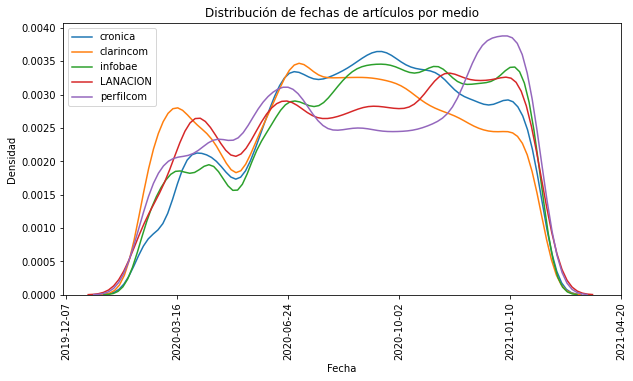
\includegraphics[width=\textwidth]{img/fechas_por_medios_todas.png}
    \caption{Distribución temporal de artículos recolectados}
    \label{fig:fecha_articulos_por_medio_todas}
\end{figure}



\begin{figure}
    \centering
    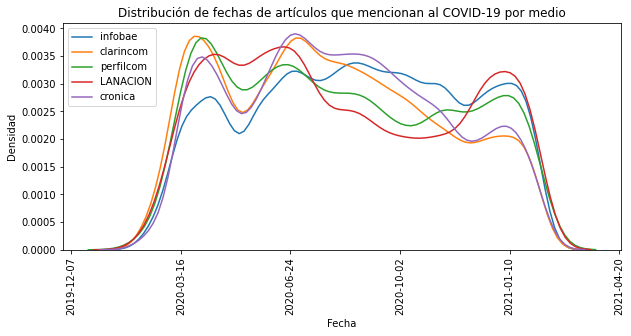
\includegraphics[width=\textwidth]{img/fechas_por_medios.png}
    \caption{Distribución temporal de artículos recolectados que mencionan COVID-19 o algún término relacionado}
    \label{fig:fecha_articulos_por_medio_covid}
\end{figure}



\section{Selección de datos a anotar}


Un problema que se nos presenta antes de comenzar el etiquetado es el de seleccionar los artículos que vamos a etiquetar. Una primera posibilidad para hacer esto es realizar una selección aleatoria de artículos y comentarios; sin embargo, los comentarios discriminatorios no se distribuyen de manera uniforme entre los artículos, sino que se concentra en algunos temas. Es mucho más probable encontrar comentarios de índole discriminatoria en notas que tengan temas cercanos a alguna de las características protegidas; por ejemplo, es esperable que encontremos contenido odioso en notas sobre China y el Coronavirus o sobre una chica transgénero antes que en un artículo de fútbol o economía.

Teniendo esto en cuenta, evaluamos varias alternativas. La primera es observar los artículos e intentar seleccionar aquellos que consideremos que puedan tener contenido potencialmente discriminatorio.

Una posibilidad para esto sería usar algunas palabras ``semilla'' para seleccionar artículos interesantes. Otra sería buscar directamente comentarios que contengan algunos insultos comunes o expresiones peyorativas hacia nuestros grupos protegidos. Después de algunos experimentos, decidimos utilizar el muestreo basado en comentarios.

\subsection{Selección en base a artículos}

En primer lugar, consideramos la posibilidad de hacer una selección en base al contenido de los artículos. Luego de realizar algunos experimentos usando LDA \cite{blei2003latent} para buscar tópicos posibles de las notas, decidimos realizar una selección un poco más controlada y determinística en base a la utilización de palabras clave. Es decir, seleccionaremos artículos en base a la aparición o no de ciertas ``semillas''

Para ello, indexamos todos nuestros artículos en MongoDB \footnote{\url{https://www.mongodb.com/}}, una base de datos no relacional y desestructurada. MongoDB permite la utilización de índices en base a texto, y realizar búsquedas en base a textos, palabras, e inflexiones. Cada artículo fue indexado en base al contenido de su cuerpo (es decir, el texto en sí del artículo).

La tabla \ref{tab:palabras_articulos} muestra el conjunto utilizado para recolectar artículos. Como vemos, hay diversas palabras que recogen distintas temáticas de posibles tópicos ``calientes'', algunos muy locales respecto a eventos concretos durante la pandemia. Si algún artículo contiene una de las frases mencionadas, se selecciona el artículo para ser etiquetado.

\begin{table}[]
    \centering
    \begin{tabular}{l | l | l | l}
    China        &  piqueteros              &  mamá                & empleadas domésticas  \\
    Cuba         &  villas                  &  de género           & la modelo             \\
    cubano       &  la villa                &  aborto              & la periodista         \\
    bolivia      &  movimientos sociales    &  actriz              & la cantante           \\
    paraguayo    &  organizaciones sociales &  actrices            & travesti              \\
    judío        &  tomas de tierras        &  feminista           & trans                 \\
    camionero    &  toma de tierras         &  femicidio           & gay                   \\
    ladrón       &  sindicatos              &  enfermera           & homosexual            \\
    represión    &  Guernica                &  madre               & de la V               \\
    criminal     &  mapuches                &  personal doméstico  & Ofelia                \\
    \end{tabular}
    \caption{Palabras utilizadas para la selección de artículos}
    \label{tab:palabras_articulos}
\end{table}

\subsection{Selección en base a comentarios}

Otra posibilidad evaluada fue la de observar los comentarios de los artículos en lugar del contenido del artículo, y seleccionarlos en base a esto. En este punto, la idea es únicamente seleccionar los artículos y no los comentarios; estos últimos son sólo usados como ``pistas'' para ver comentarios con posible contenido discriminatorio, y como tal identificar a ese artículo como un posible generador de este tipo de contenido.

La idea es similar a la de la selección con artículos, sólo que aplicada a comentarios: buscamos comentarios que contengan alguna de las palabras semilla listadas en la Tabla \ref{tab:palabras_comentarios}. Estas palabras fueron recolectadas a base de experimentación y observación de los datos, y tratan de contener diversas expresiones de contenido mayormente discriminatorio.

Una idea también considerada fue la de utilizar un clasificador entrenado sobre otro dataset (por ejemplo, el de \citet{hateval2019semeval}) y con eso marcar comentarios posiblemente discriminatorios. Sin embargo, muy probablemente detectaríamos sólo comentarios para las categorías/características etiquetadas en esos datasets e ignorarían las que agregamos en nuestro trabajo; por ejemplo, la mayoría de los datasets no contienen comentarios anotados contra la comunidad LGBTI.

El procedimiento de selección consta de, dado un artículo, marcar sus comentarios que contengan una o más de las expresiones listadas. Si el artículo tiene tres o más comentarios marcados, entonces seleccionamos el artículo; caso contrario, es descartado.

\todo{Agregar comparación con métodos de recolección en base a esto de 'seed' words}

Vale remarcar que este proceso de selección es para los \emph{artículos}, no para los comentarios.

\begin{table*}[t!]
    \centering
    \begin{tabular}{l|l|l|l|l|l|l}
    bija          & urraca     & viejo puto    & trolo      & peruano  & matarlos         & negra      \\
    prostituta    & tucán      & trabuco       & sodomita   & peruca   & una bomba        & negro de   \\
    feministas    & putita     & travesti      & chinos de  & judío    & vayan a laburar  & negros     \\
    feminazis     & reventada  & trava         & bolita     & sionista & vayan a trabajar & bala       \\
    aborteras     & marica     & degenerado    & paraguayo  & villeros & gorda            & uno menos  \\
    \end{tabular}
    \caption{Palabras utilizadas para recolectar comentarios}
    \label{tab:palabras_comentarios}
\end{table*}

Luego de algunos análisis experimentales y observacionales de las dos posibles metodologías, decidimos utilizar el muestreo de artículos en base a comentarios. En base a un análisis subjetivo, los artículos seleccionados parecían tener mayor incidencia de mensajes odiosos y eso nos decantó hacia esa opción.

\section{Criterios de anotación}
\label{sec:criterios}

La definición de lenguaje discriminatorio utilizada en este trabajo está basada en trabajos de la Comisión Interamericana de Derechos Humanos (CIDH)\cite{CIDH2015}, del Centro de Estudios de Libertad de Expresión (CELE) \cite{cele2019} y en el Article 19 Hate Speech Toolkit \cite{article192015}.

Teniendo estos insumos en cuenta, entendemos que hay discurso discriminatorio en un texto social si contiene declaraciones de carácter intenso y posiblemente irracional de rechazo, enemistad y aborrecimiento contra un individuo o contra un grupo, siendo estos objetivos de estas expresiones por poseer (o aparentar poseer) una característica protegida.

Las características en cuestión son protegidas por leyes internacionales. En este trabajo consideramos las siguientes:

\begin{enumerate}
\item Sexo (Mujeres, concretamente)
\item Género o identidad sexual (Colectivo LGBTI)
\item Ser inmigrantes, extranjeros, pueblos aborígenes u otras nacionalidades (xenofobia, racismo)
\item Situación socioeconómica o barrio de residencia
\item Poseer discapacidades, problemas salud mental o de adicción al alcohol, drogas u otros estupefacientes
\item Opinión o ideología política
\item Aspecto o edad (mayormente, gordofobia/gerontofobia)
\item Antecedentes penales o estar privado de la libertad
\end{enumerate}

Si bien algunas de estas características no son consideradas en algunos tratados (por ejemplo, contra los presos), las tuvimos en cuenta por las características propias del tratamiento en medios durante la pandemia de distintos sucesos.

\todo{Linkear el apéndice}

\section{Modelo de etiquetado}



Un modelo de anotación es, según \citet{pustejovsky2012natural}, una representación práctica del objetivo de anotación. En nuestro caso, queremos marcar comentarios discriminatorios, marcar a qué grupos y/o características se está ofendiendo, y también identificar llamados a tomar alguna acción contra los objetos de esos discursos. Por lo pronto, haremos una definición que capture ese objetivo sin deternos demasiado en especificarlo formalmente (lo que llaman en ese libro ``especificación'').

\subsection{Modelo Jerárquico de Etiquetado}



\begin{figure}
    \centering
    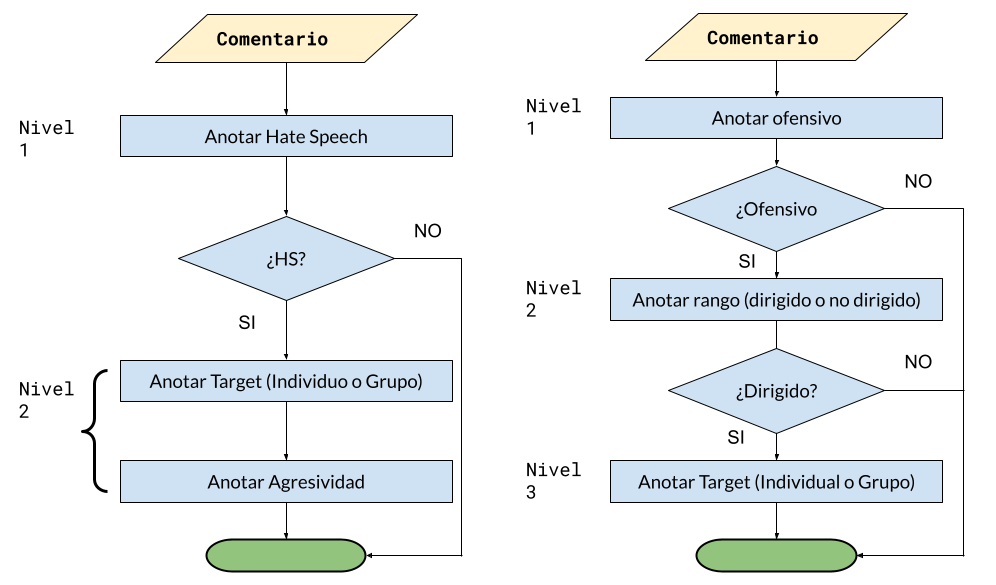
\includegraphics[width=\textwidth]{img/modelosjerarquicos.png}
    \caption{Modelos jerárquicos de anotación. A la izquierda, tenemos el modelo jerárquico propuesto para HatEval \cite{hateval2019semeval}, a la derecha el modelo propuesto para OffensEval \cite{zampieri2019semeval2019}}
    \label{fig:modelos_offenseval_hateval}
\end{figure}

\subsection{Modelo de etiquetado jerárquico y contextualizado}

\citet{zampieri2019predicting} introdujeron un modelo jerárquico de anotación para la tarea de lenguaje ofensivo, utilizado en las competiciones OffensEval \cite{zampieri2019semeval2019} y hatEval \cite{hateval2019semeval}. La idea de la anotación jerárquica es realizar anotaciones adicionales sólo para algunos casos de anotaciones del nivel anterior.

En el caso de \emph{HatEval}, tenemos un primer nivel que consta de anotar si un tweet contiene o no lenguaje de odio (nivel 1). Si el tweet tiene lenguaje de odio, entonces anotamos si está dirigido a un individuo o a un grupo, y también anotamos si es agresivo o no (ambos nivel 2). En el caso de \emph{OffensEval}, primero anotamos si es ofensivo (nivel 1), luego si está dirigido o es un insulto no dirigido (nivel 2) y finalmente, si es dirigido y ofensivo, marcamos su objetivo (nivel 3). En la figura \ref{fig:modelos_offenseval_hateval} ilustramos ambos modelos.


%
%
% Link: https://docs.google.com/drawings/d/1ZgTmvRwMWn0B-kokfw87jfSa7eY5-OSBHwltetnNT08/edit
%



\begin{figure}
    \centering
    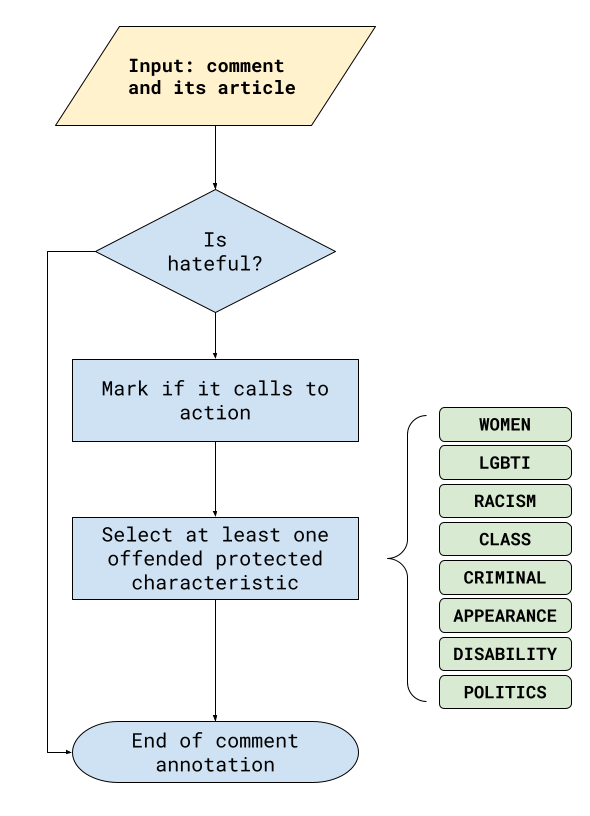
\includegraphics[width=0.5\textwidth]{img/Annotation Model.png}
    \caption{Modelo de anotación}
    \label{fig:annotation_model}
\end{figure}


La figura \ref{fig:annotation_model} muestra el modelo de anotación utilizado para el dataset construído en este trabajo. Seguimos un modelo jerárquico similar al propuesto por \citet{zampieri2019predicting}, aunque de sólo un nivel. Para cada comentario y su respectivo contexto (el artículo), requerimos una anotación  para decidir si el comentario es odioso o no. Si no es odioso, no se necesita más información. Si es así, el par artículo-comentario debe contener, además, una anotación por si llama o no a la acción, y al menos una categoría protegida





\section{Etiquetadores}

A diferencia de otros trabajos (como hatEval \cite{hateval2019semeval}), decidimos por un lado, garantizar que nuestros anotadores estén más cercanos culturalmente al problema en cuestión, a la vez que tener mayor control del perfil de estos. Consideramos que el discurso de odio tiene un fuerte componente cultural, muchas veces expresado a través de jerga o expresiones dialectales muy particulares, y relacionado con noticias muy propias de esta región.


\subsection{Tipos de anotación en otros trabajos}

Comentar otros trabajos acá

\begin{itemize}
    \item Davidson
    \item Waseem
    \item hatEval
    \item CONAN
    \item Gao (contextualizado)
    \item Context offensive (el de Google, y el griego)
\end{itemize}

\subsection{Perfil de etiquetadores}

Para la selección de anotadores, realizamos una búsqueda interna. Puntualmente, buscamos:

\begin{itemize}
    \item Estudiantes/graduades de carreras de Cs. Sociales, Psicología, Letras o afines
    \item Hablantes nativos (o casi) de Español Rioplatense
    \item Usuarios de redes sociales; preferentemente Twitter
\end{itemize}

Luego de una breve entrevista donde les contamos el proyecto y corroboramos que efectivamente sean hablantes nativos de Español Rioplatense y usuarios de RRSS, les mandamos una pequeña evaluación paga que constó de leer el manual de criterios de anotación (que agregamos en \ref{app:manual_criterios_anotacion}) y anotar 5 artículos. Esto lo realizamos para ver que efectivamente estén entendiendo la tarea. Estos artículos fueron luego reutilizados para el proceso de entrenamiento.

\section{Proceso de etiquetado}

\subsection{Preprocesado y filtrado de los datos}

El preprocesado de los datos es muy básico: en los hechos, efectuamos el mismo preprocesamiento que en anteriores tareas, consistente en reemplazar handles de Twitter por un token especial \verb|@usuario| para evitar cualquier sesgo. Por ejemplo, si un usuario conocido como ``odiador'' (llamemos \verb|@hater|) retwittea la noticia y otro responde a ese RT, aparece ese nombre de usuario lo cual podría condicionar al etiquetador.

Así mismo, descartamos cualquier tweet que tuviera algún link ya que pueden referir a contenido no textual


\subsection{Entrenamiento de etiquetadores}



%
% Esto quizás va después
%
\subsection{Herramienta de etiquetado}

%%
%% Link a Google Draw: https://docs.google.com/drawings/d/1E24-2l6hsNj2JSKBZOD8QvZCJR6rrGjz-cWwt8XuPRg/edit
%%

\begin{figure}
    \centering
    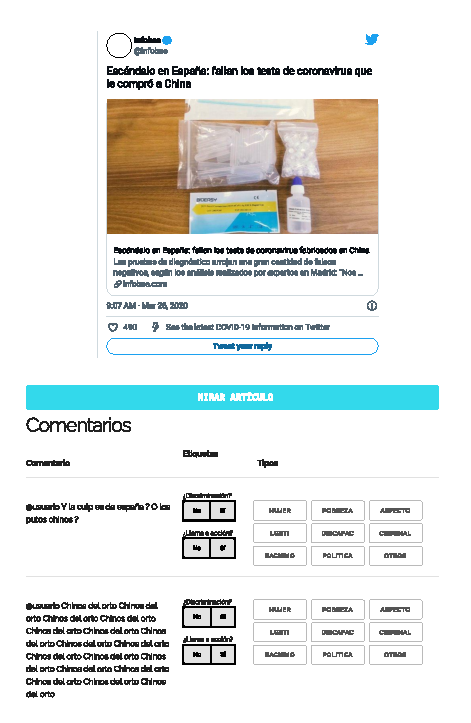
\includegraphics[width=\textwidth]{img/labeler.pdf}
    \caption{Pantalla del etiquetador}
    \label{fig:labeler_example}
\end{figure}

Al no utilizar ningún servicio de etiquetado, optamos por desarrollar nuestra propia aplicación para el etiquetado de tweets. En ella, a cada etiquetador les fueron asignados progresivamente los artículos a anotar, los cuales fueron agrupados en ``lotes'' para facilitar la tarea administrativa de la asignación.

La figura \ref{fig:labeler_example} muestra la interfaz presentada a los etiquetadores. Cada artículo es presentado al etiquetador junto a los comentarios asignados. Ante esto, el etiquetador puede elegir saltear el artículo o etiquetarlo. Si decide etiquetarlo, el etiquetador debe para cada comentario marcar usando un control de tipo ``switch''

\begin{enumerate}
    \item Si el comentario contiene discurso discriminatorio
    \item En caso de ser discriminatorio, marcar si llama a la acción
    \item En caso de ser discriminatorio, marcar al menos una característica ofendida
\end{enumerate}

Para el desarrollo de la aplicación usamos Django\footnote{\url{https://www.djangoproject.com/}}, un framework de python para desarrollo web, y Javascript plano. Como base de datos utilizamos SQLite ya que tenía una baja tasa de concurrencia (sólo 6 usuarios.)

\subsection{Esquema de anotación}

%Teniendo en cuenta el modelo de anotación ilustrado en la figura \ref{fig:annotation_model}, optamos por la siguiente metodología para el etiquetado de los comentarios de nuestro dataset.

%%
%%
%% Link a Google Draw:
%% https://docs.google.com/drawings/d/1esS9tAwpPVydohxd-B-xwVdAaPQRVGAo0MruBrgSKig/edit
%%
%%

\begin{figure}
    \centering
    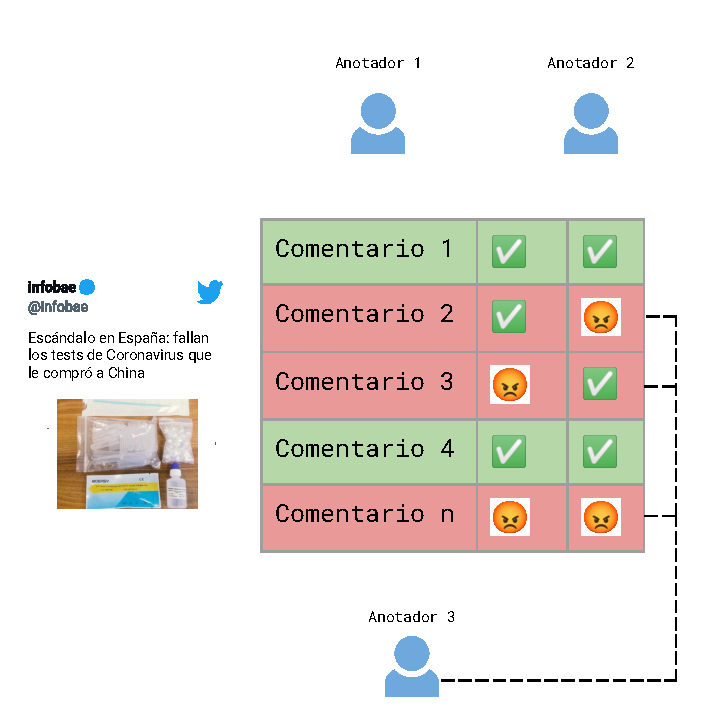
\includegraphics[width=0.7\textwidth]{img/esquema_anotacion.pdf}
    \caption{Esquema de anotación. Caso en que ambos anotadores etiqueten los comentarios del artículo}
    \label{fig:annotation_schema}
\end{figure}

Los artículos son asignados a cada etiquetador. Cada etiquetador, al serle presentado un artículo, tiene dos opciones: etiquetarlo o saltearlo. La idea de saltear era doble: evitar contenido poco ``interesante'' en términos de comentarios discriminatorios, o evitar contenido sensible para el anotador (algo que no ocurrió afortunadamente).

Una posibilidad que barajamos en un principio fue asignar para el etiquetado el artículo completo a 3 anotadores. Sin embargo, esta modalidad sería altamente ineficiente dada la baja cantidad de contenido discriminatorio. Entonces, decidimos ir por un esquema de ``desempate'': dos anotadores anotan un artículo, y luego un tercero anota sólo aquellos donde al menos uno marcó que es discriminatorio. Esto da la posibilidad de que haya una tercera anotación incluso cuando dos previas marcaron que el comentario es discriminatorio, y lo hacemos para recolectar más información. \todo{marcar otros trabajos que hayan hecho esto}. Con este esquema de anotación, y teniendo en cuenta los números finales obtenidos del dataset, dedicamos 2.16 etiquetados por comentarios versus 3 etiquetados por comentario de anotar tres veces todo. La figura \ref{fig:annotation_schema} ilustra este flujo de anotación.

Entonces, en primer lugar cada artículo es asignado a 2 anotadores. Luego de esto, se solicita una tercera anotación pero sólo sobre los comentarios que tengan alguna de las dos etiquetadas marcando contenido discriminatorio, y no dando la posibilidad de saltear. Ahora ¿qué pasa si alguno de los dos anotadores saltea el artículo?. Tenemos dos casos. Si los dos saltean el artículo, entonces descartamos ese artículo. Ahora, puede ocurrir el caso de que uno lo saltee y el otro lo anote: en ese caso, y en pos de maximizar el contenido discriminatorio encontrado o uno lo hace y el otro anota menos de 4 comentarios odiosos, entonces no pasa a 3ra anotación y lo descartamos del dataset. Si uno salteó y el otro anotador anotó 4 o más comentarios odiosos, entonces forzamos al primer anotador a anotar el artículo, sin dar esta vez opción de saltear. La figura \ref{fig:annotation_schema_case_two} ilustra el flujo para este caso.


%%
%%
%% Link a Google Draw
%% https://docs.google.com/drawings/d/1TOlCgZggCmYHgZWV7ZrIIlXuhcFUMeYw4PcFM7XdY2k/edit
%%
%%

\begin{figure}
    \centering
    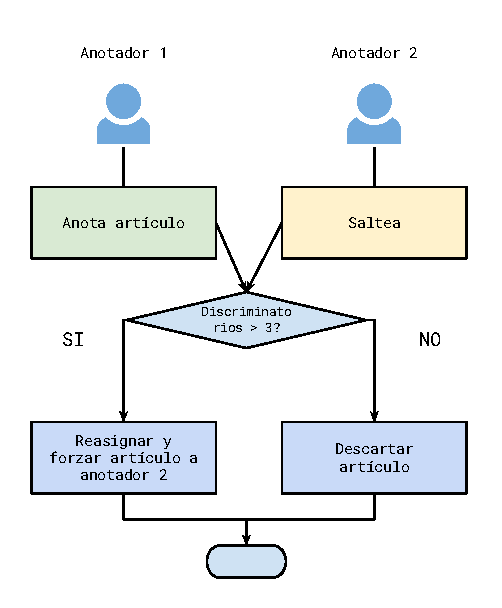
\includegraphics[width=0.6\textwidth]{img/esquema_anotacion_caso_2.pdf}
    \caption{Esquema de anotación. Caso en que un anotador saltee}
    \label{fig:annotation_schema_case_two}
\end{figure}


Como resultado de este esquema, cada comentario de nuestro dataset puede tener dos o tres anotaciones, siendo los casos posibles los siguientes:

\begin{enumerate}
    \item Dos anotaciones negativas
    \item Tres anotaciones, siendo al menos una que marque el comentario como discriminatorio
\end{enumerate}




\subsection{Asignación}

\citet{pustejovsky2012natural} denominan ``asignación'' al procedimiento de extraer las ``gold labels'' de las etiquetas. En este punto tenemos una etiqueta binaria si el contenido es discriminatorio o no (notamos HS) en el primer nivel, y luego 9 etiquetas binarias: una para la llamadas a la acción (CALLS) y otras 8 para las características ofendidas. Recordemos que una anotación negativa sólo consta de HS negativo, mientras que una positiva consta de un HS positivo, una etiqueta para CALLS y al menos una etiqueta positiva de las características restantes.

Para este dataset, tomamos las siguientes decisiones:

\begin{enumerate}
    \item Para la etiqueta de HS, realizamos la votación mayoritaria
    \item Si hay HS, CALLS es positivo sii es votación mayoritaria
    \item Si hay HS, marco como positivas todas aquellas características marcadas por los anotadores
\end{enumerate}

La primer decisión es la más obvia y razonable, pero las otras dos decisiones merecen alguna discusión. Para que sea un comentario considerado como HS, tiene que ocurrir que al menos dos etiquetadores lo marquen como tal. En ese caso, para que haya votación mayoritaria de CALLS, tiene que haber dos o más votos marcados como tal; en caso de empate, es decir, que un anotador marca que hay llamado a la acción y otro que no, marcamos que no hay llamado a la acción.

En el caso de las características, marcamos todas las que hayan marcado aquellos anotadores que hayan etiquetado HS. Esta decisión podría haberse tomado de otra manera; por ejemplo, sólo tomando aquellos casos donde haya cierto grado de coincidencia entre los comentarios. Sin embargo, al considerar que los límites entre las características son difusos (por ejemplo, apariencia y mujer tienen un grado de coincidencia, y a veces clasismo y racismo también) preferimos optar por este esquema.

\todo{Agregar algún gráfico de esto}

\subsection{Recursos utilizados}

El etiquetado constó de XXX horas. A cada etiquetador le fue pagado YYYY por hora, y luego ZZZ por hora en segunda instancia. Esto equivale a WWW USD.

\section{Dataset resultante}

\begin{table}
    \centering
    % \begin{tabular}{lrr}
    %     \toprule
    %     Total articles & 1238    \\
    %     Total comments &  56869  \\
    %     Hateful Tweets &   8715  \\
    %     Ratio          &   0.153 \\
    % \end{tabular}
    \begin{tabular}{lrr}
        \toprule
        Característica &  Count &  Calls to Action \\
        \midrule
        RACISM         &   2469 &              674 \\
        APPEARANCE     &   1803 &               34 \\
        CRIMINAL       &   1642 &              722 \\
        POLITICS       &   1428 &              136 \\
        WOMEN          &   1332 &               18 \\
        CLASS          &    823 &              135 \\
        LGBTI          &    818 &               11 \\
        DISABLED       &    580 &                4 \\
        \bottomrule
    \end{tabular}
    \caption{Figures of the annotated dataset, by total numbers and segmented by characteristic}
    \label{tab:dataset_figures}

\end{table}

El dataset resultante consta de 1238 artículos etiquetados, y 56869 comentarios respectivamente, de los cuales 8715 contienen contenido discriminatorio según los criterios de asignación antes referidos. Podemos observar que aproximadamente 1 de cada 6 comentarios es discriminatorio; esto no es representativo del universo de notas periodísticas ya que recordemos que la selección de los datos no fue aleatoria. La tabla \ref{tab:dataset_figures} contiene estos datos estadísticos.

De todos los tweets discriminatorios, tenemos en particular los llamados a la acción. La inmensa mayoría de estos está dirigido hacia la categoría CRIMINAL, muchos en la forma de llamados a matar a criminales y otros delincuentes.

La tabla \ref{tab:annotation_agreement} reporta el acuerdo entre anotadores usando la métrica alpha de Krippendorff \todo{agregar cita}. Reportamos el valor de $\alpha$ para HS sobre todas las etiquetas, y luego todas las etiquetas del segundo nivel del modelo jerárquico (características y llamado a la acción) sólo sobre aquellas que hayan marcado que el comentario contiene HS. Esto es equivalente a calcular el acuerdo con una etiqueta faltante en el segundo nivel para las características y el llamado a la acción. Si bien este acuerdo tiende a ser alto, debe leerse como el acuerdo sobre la razón detrás del hate speech; la mayor penalización queda reservada a HS, que tiene $\alpha = 0.59$, algo que podría marcarse como un buen acuerdo teniendo en cuenta los parámetros vistos en las tablas de preliminares. \todo{linkear esto}

\begin{table}
    \centering
    \begin{tabular}{lc}
        \toprule
        Categoría   & $\alpha$ de Krippendorff \\
        \midrule
        Hateful              &  0.579 \\
        Calls to Action      &  0.641 \\
        \midrule
        WOMEN                &  0.783 \\
        LGBTI                &  0.920 \\
        RACISM               &  0.929 \\
        CLASS                &  0.706 \\
        POLITICS             &  0.808 \\
        DISABLED             &  0.849 \\
        APPEARANCE           &  0.871 \\
        CRIMINAL             &  0.931 \\
        \bottomrule
    \end{tabular}
    \caption{Reported Agreements. \emph{Hateful} agreement is reported for the binary decision of a tweet assigned as hateful or not; for the other characteristics (and the calls to action) the agreement is calculated over those tweets with two or more hateful marks}
    \label{tab:annotation_agreement}
\end{table}

\subsection{Análisis por característica}

En la tabla XXX podemos observar algunos ejemplos seleccionados de comentarios. Algunas observaciones que pueden realizarse es que los comentarios marcados contra las mujeres tienen en algunos casos ciertas complejidades, como las acusaciones de ``mentirosa'' a una mujer que sufrió una violación (caso Thelma Fardin \todo{Agregar nota de esto}), apreciaciones a su cuerpo, entre otras cosas.

Una categoría desafiante pareciera ser los comentarios discriminatorios contra la comunidad LGBTI. Más allá de algunos insultos explícitamente ofensivos (mediante insultos del estilo trolo, trabuco, maricón, etc), hay muchos que tienen un contenido difícil de descifrar; en particular, aquellos comentarios contra personas trans. Muchos de estos mensajes hacen alusiones a su genitalidad o a su cuerpo en general, de manera metafórica o irónica, lo cual hace verdaderamente difícil su detección. A su vez, es claro que en muchos de estos comentarios es sumamente necesaria la información contextual para poder comprender el caracter abusivo de estos comentarios.

En el caso de la categoría CRIMINAL, se puede observar por un lado comentarios muy violentos (``bala'', ``mátenlos'', ``plomo'') que necesitan el contexto para entenderse como ofensivos contra esa característica (por ejemplo, si la nota fuese sobre una plaga de mosquitos no deberíamos considerarlo como ``discriminatorio''). Por otro lado, algunos comentarios son más difíciles de descifrar y dependientes del contexto, como las celebraciones ante el abatimiento de un preso o criminal (``bravo'', ``felicitaciones!'') que parecen inofensivas hasta que se lee el contexto de la noticia. De hecho, a diferencia de otros comentarios, parecen tener hasta una polaridad positiva.

En el caso de racismo (la categoría más marcada del dataset) hay una fuerte cantidad de comentarios discriminatorios contra la comunidad china. Esto es esperable por el brote racista debido a la pandemia del COVID-19, documentado en YYYY \todo{agregar cita}. Así mismo, es de las categorías que más llamados a la acción tiene, muchos del estilo de tirar bombas, aniquilar, etc a China o a la comunidad de dicho país, o llamados a tomar medidas ``blandas'', como ``no ir a comprarles a los supermercados''.

Algunas de las categorías tienen características más elementales, como política, apariencia, y discapacidad. En los comentarios ilustrados. Esto es esperable ya que

Algunas de las agresiones, a su vez, usan técnicas de camuflaje (``tafaldegaver'', falta de verga, ``docer''), que dificultan su detección por las técnicas actuales.

\begin{table}
    \scriptsize
    \centering
    \begin{tabular}{p{0.1\textwidth} p{0.45\textwidth} p{0.40\textwidth}}
        \hline
        Tipo & Contexto & Texto \\
        \hline
        %WOMEN & Nicole Neumann apuntó contra los consumidores de carne: “Sigan comiendo asadito” & @usuario Debieras comerte uno así te sacas esa cara agria que tenes🤣🤣👎 \\
        \mr{12}{MUJER} & Por el mundo: Florencia Peña mostró su lujosa nueva casa con bar, muelle y pileta & @usuario Cuando succionas las correctas \\
         & El exabrupto de Rodolfo Barili con una modelo que se metió en el baúl de un auto para violar la cuarentena & @usuario Barili, ojo es mujer, en cualquier momento te caen las hordas de feminazis, pero estoy al 100\% CON VOS!! \\
         & Video: tres mujeres forzaron la puerta de un edificio en Palermo y desvalijaron dos departamentos & @usuario 3 feministas , claramente es el perfil de las feministas \\
         & Británica llegó a Perú por 10 días y se quedó por amor: vive sin agua potable y entre insectos & @usuario Pero empomada todo el día... \\
         & “Me esterilicé, pero no odio a los niños”: mi vida dentro del movimiento “libre de hijos” & @usuario Es que sos incogible..quien te va a hacer un hijo.....algun ciegoooo \\
         & Mia Khalifa: actuó en videos porno durante pocos meses, cobró fama mundial y ahora lucha por borrar su pasado & @usuario JAJAJAJAAJAJAAJA SEGUILA CHUPANDO.... \\
         & ¿Se puede ser feminista y llorar a Diego Maradona? & @usuario Para las feminazis toda ilógica es correcta \\
         & Claribel Medina, indignada con un grupo de personas reunidas en un bar: “La gente está sin barbijo mientras los actores no podemos trabajar” & @usuario La menopausia nos pone locas 🤦🏽‍♀️🤣 \\
         & Narda Lepes: “Mil veces me tocaron el culo en las cocinas de los restaurantes” & @usuario Tenes lindo culo? \\
         & Un policía se defendió de un robo en Pompeya, mató a un ladrón y estuvo dos días preso & @usuario Que jueza hija de mil puta ojalá t afanen a vos y t maten un ser querido a ver qué haces LLEGUA de mierda puta \\
         & “Cristian, mirá lo que hago por vos”: quién es la modelo que se metió en el baúl de un auto para violar la cuarentena & @usuario Jajaja modelo Hot jaja Telosu!! Mami diría la Moria !! Jaja ridícula tafaldegaver \\
         & La aberrante arenga machista que dio el preparador físico de Güemes de Santiago del Estero & @usuario Que aliade te volviste Clarín, vos te culeas la que tiene olor a pingo (feminazi) \\
        \hline
        \hline
        \mr{8}{LGBTI} & Por qué Flor de la V no continuó en Mujeres de eltrece, tras la salida de Claudia Fontán & @usuario y..porque no es mujer, más claro echale agua \\
         & Histórico: Mara Gómez fue habilitada y será la primera jugadora trans en el fútbol argentino & @usuario Unos huevos bárbaros tiene esta mina!!!!! \\
         & La historia de la modelo colombiana trans que besa la panza de su esposo embarazado de ocho meses & @usuario Un macho besando a otro macho \\
         & Luis Novaresio le dedicó un romántico mensaje a Braulio Bauab por su cumpleaños & @usuario Guacale \\
         & Eugenio Zaffaroni le contestó a Sergio Berni tras la polémica por las domiciliarias: “Es el populacherismo vindicativo que llenó las cárceles” & @usuario cuando se muere este viejo trolo enfermo \\
         & La impactante historia de la tenista trans que hoy es la N° 3 de Argentina en la categoría senior femenino & @usuario Vergonzoso que  las mujeres toleren esto.\textbackslash nEse tenista debería jugar con hombres o a lo sumo, en un torneo de sujetos como él. \\
         & Joe Biden nominó a Rachel Levine, una mujer transgénero, para que sea su subsecretaria de Salud & @usuario Este presidente es la dejeneracion total del mundo \\
         & Así luce el actor Elliot Page tras declararse trans & @usuario Tiene Bija? No. Tiene Concha? Si. Es mujer entonces \\
         & El abuelo que a los 90 años confesó: “Soy gay, soy libre y estoy afuera” & @usuario Como no te agarra el Coronavirus.   🤮🤮 \\
        \hline
    \end{tabular}

    \caption{Ejemplos discriminatorios del dataset contra mujeres y la comunidad LGBTI.}
    \label{tab:women_and_lgbti_examples}
\end{table}


\begin{table}
    \scriptsize
    \centering
    \begin{tabular}{p{0.1\textwidth} p{0.45\textwidth} p{0.40\textwidth}}
        \hline
        Tipo & Contexto & Texto \\
        \hline
        \mr{9}{RACISMO} & Coronavirus: las terribles imágenes del mercado donde se originó la pandemia & @usuario Hay que matarlos hijos de puta 😑 \\
         & Malestar en Washington con el Gobierno argentino porque no dejó atracar al buque más moderno de la guardia costera de Estados Unidos & @usuario Amo ver los sudacas que se creen yankis enojados por esto. \\
         & Milagro Sala: “Seguimos presos, los que nos gobiernan tienen que cambiar las cabezas” & @usuario Negra, seguis presa por chorra. \\
         & Al menos 7 muertos en China a causa de un virus transmitido por garrapatas & @usuario Que no venga ningún chino más a la Argentina! Por favor! Ya Basta! \\
         & En China comenzó el tradicional Festival de Carne de Perro a pesar de la pandemia de coronavirus y una ONG intenta salvarlos & @usuario No soy racista, pero hay que matar a todos los chinos \\
         & Científicos identificaron en China otro virus respiratorio “con potencial para convertirse en pandemia” & @usuario Nos infectan a Todos!!! \\
         & Coronavirus. Yanzhong Huang: "Es bastante probable que ya se esté gestando un Covid-21" & @usuario Bombas urgente a esta maldita raza \\
         & Denunciaron la nueva maniobra de China para ocultar las verdaderas cifras del coronavirus & @usuario Mundialmente mantenemos china xq todo viene de ahí y hoy estamos fundidos y en emergencia... \#ChinaVirus no quiero ver un \#chino x mucho tiempo! \\
         & Villa Mascardi: impresionante operativo con tanquetas blindadas para que una fiscal ingresara a una zona controlada por mapuches & @usuario Basta!!! No son mapuches son delincuentes !!! A ver si alguien pone las pelotas donde hay que ponerlas y los cagan a tiros de una vez !!! \\
        \hline
        \hline
        %\rotatebox[origin=c]{90}{rota}
        \mr{5}{CRIMINAL} & Aberrante: un político de Misiones admitió haber esclavizado y violado a sus tres hijastras & @usuario Solo se requiere una bala. \\
         & Rosario: un grupo de vecinos linchó y mató a golpes a un joven acusado de robar autos & @usuario esta perfecto, ejemplo a los demás \\
         & El panadero que mató a un ladrón en La Matanza: "No soy un asesino, estoy arrepentido" & @usuario Que dice señor ! No sé arrepienta, que hizo una obra de bien.Era su vida o la del delincuente. \\
         & Video: salió de la cárcel por el coronavirus y murió de un tiro el mismo día al festejar su libertad & @usuario Justicia divina!! \\
         & Le sacó el arma al ladrón que lo asaltó, lo corrió y lo mató de un disparo: quedó detenido & @usuario Buenísimo vamos por el exterminio total de estos primates. \\
        \hline
        \hline
        \mr{8}{CLASE} & La Justicia ordenó el desalojo de la masiva toma de terrenos en Guernica & @usuario Lanzallamas y a otra cosa \\
         & Hubo tensión en la Quinta de Olivos entre un grupo que apoyaba a Alberto Fernández y manifestantes del banderazo contra el Gobierno & @usuario PLANEROS Y BARRABRAVAS \\
         & Organizaciones sociales cortaron la avenida 9 de Julio: reclamaron un salario mínimo de \$ 45.000 & @usuario Vayan a lo laburar hdp. \\
         & La historia de una familia de cartoneros en la toma de Guernica: “Por primera vez sentimos que tenemos un hogar” & @usuario Bala. \\
         & El Gobierno autorizó la apertura de las escuelas porteñas para las elecciones de Bolivia & @usuario No sería mejor deportar a los bolivianos indocumentados?.además nos suman pobreza e indigencia \\
         & Coronavirus en Argentina: un dirigente radical deseó que la pandemia “haga una limpieza étnica” con “negros de La Matanza” & @usuario Es el deseo de todo argentino de bien \\
         & El Polo Obrero realiza un corte en la Panamericana en contra de la flexibilización de la cuarentena y en reclamo de aumentos a los planes sociales & @usuario Clarísimo que no quieren laburar y quieren vivir de nosotros! \\
         & Coronavirus en la Argentina: movimientos sociales reclaman asistencia alimentaria en el Obelisco & @usuario Anda a laburar lpqtp \\
        \hline
    \end{tabular}

    \caption{Ejemplos discriminatorios del dataset por motivos de clase, racismo, o contra criminales.}
    \label{tab:class_racism_examples}
\end{table}


\begin{table}
    \scriptsize
    \centering
    \begin{tabular}{p{0.1\textwidth} p{0.45\textwidth} p{0.40\textwidth}}
        \hline
        Tipo & Contexto & Texto \\
        \hline

     \mr{5}{POLITICA} & Confirman una mutación en el coronavirus que puede hacerlo 10 veces más contagioso que la cepa original de Wuhan & @usuario ME ALEGRO MUCHÍSIMO.\textbackslash nOJALÁ LLEGUE PRONTO A ARGENTINA Y ARRASE CON TODO.\textbackslash nPODRÍAMOS VER AL FIN ALGO MÁS DAÑINO QUE EL CÁNCER PERONISTA Y SU METÁSTASIS KIRCHNERISTA. \\
      & Murió un nieto recuperado por Abuelas de Plaza de Mayo: los mensajes de Alberto Fernández y Cristina Kirchner & @usuario Un planero menos. \\
      & Última encuesta: ¿Qué mujer superó a Alberto Fernández en imagen positiva? & @usuario Les ahorro el clickbait. Es Vidal, igual perdió por 20 puntos. Gorila LTA. \\
      & Cómo es la cerveza “peronista” que el Chacho Coudet le regaló a Alberto Fernández & @usuario Debe ser meo de gato. berreta como todo lo peroncho \\
      & El descargo de Nicolás Wiñazki después de que Vero Lozano se burlara de él: “Quizás le afecta la cuarentena” & @usuario Yo creo que al revés, patético operador. Solo los gorilas pueden bancarte croto \\
      \hline
      \hline
    \mr{5}{APARIENC.} & Axel Kicillof recomendó una “cuarentena previa” de 14 días para “llegar sanos a Navidad y Año Nuevo” & @usuario Chuoame la verga enano moishe \\
     & Video indignante: piba violó la cuarentena y viajó en el baúl de un taxi para ver a un chico & @usuario Habría qur buscar también y meter en cana al cirujano que le hizo la nariz!! Parece Michael Jackson la loca!!! \\
     & El senador José Mayans defendió a Gildo Insfrán: “En pandemia no hay derechos” & @usuario Volve al gancho , docer \\
     & El video sexy de More Rial en corpiño & @usuario Asco \\
     & El sensual paseo en moto de Florencia Peña: "Próxima parada: tu casa" & @usuario Que tiene de sensual, ésta vieja cascoteada?prostituta de cuarta,kukaracha inmunda! \\

    \hline
    \hline
    \mr{4}{DISCAPAC.}& Patricia Bullrich pidió ser drásticos con los docentes: “El que no va, tendrá que ser reemplazado” & @usuario Estragos del tinto \\
      & El abuelo que a los 90 años confesó: “Soy gay, soy libre y estoy afuera” & @usuario Alhzeimer o demencia senil!!!!! \\
      & Elisa Carrió dijo que “ninguna pandemia es excusa para suspender la República” y advirtió que “vienen por los campos” & @usuario Si sacan a la paciente psquiatrica es porque están hasta las manos.\textbackslash n\#CarcelACambiemos \\
      & Florencia Kirchner y su posteo a favor de la amistad: "Nunca entendí la desesperación por la pareja" & @usuario La enfermita está mejor que yo,y no se calienta por la hija \\
    \hline
    \mr{6}{INCITACIÓN} & Harán un listado de los presos en situación de riesgo por el coronavirus para evaluar si deben salir de prisión & @usuario @usuario Todo al reves! Si hay alguno con coronavirus PONGANLO EN EL MEDIO! \\
         & La advertencia de Juan Grabois: “Van a haber 1, 5, 20 Guernicas” & @usuario @usuario Habra 100 paredones \\
         & Otro caso de peste bubónica enciende las alarmas en China & @usuario Una atómica a China... \\
         & Coronavirus: afirman que volvió la venta de carne de murciélagos en China & @usuario Boicot a todo producto chino!!! \\
         & Villa Mascardi: impresionante operativo con tanquetas blindadas para que una fiscal ingresara a una zona controlada por mapuches & @usuario El Diálogo se Inicia con BALAS y Finaliza con La Última \\
         & Coronavirus en China: la ciudad de Shenzhen prohíbe comer perros y gatos & @usuario habrá alguna manera de erradicar a estos tipos del mundo ? \\
    \hline
    \hline
    \end{tabular}
    \caption{Ejemplos discriminatorios del dataset. INCITACIÓN refiere a los llamados a realizar algún tipo de medida contra el grupo o la persona atacada. }
    \label{tab:politics_and_calls_examples}
\end{table}



\subsection{Anonimización para publicación de los datos}



\section{Conclusión}

En este capítulo, describimos la construcción de un dataset contextualizado de lenguaje discriminatorio o hate speech. Para ello, recolectamos respuestas a noticias periodísticas posteadas en Twitter por los principales medios de noticias de Argentina. Exploramos distintas alternativas para la selección de artículos a etiquetar, tanto observando los tópicos de los artículos como los comentarios a este. Decidimos elegir los artículos en base a sus comentarios potencialmente discriminatorios, y luego seleccionar una muestra aleatoria y acotada de comentarios.

Para realizar la tarea de etiquetado, desarrollamos nuestra propia herramienta la cual hacemos pública. Definimos un modelo de anotación jerárquico y granular para la tarea, siendo relativamente novedoso el hecho de anotar las características ofendidas en cada texto social. Seis etiquetadores nativos de la variedad dialectal rioplatense realizaron la tarea de anotación bajo un esquema de 2 anotaciones + desempate.

Como producto, obtuvimos un dataset de cerca de 57k comentarios repartidos en 1.2k artículos, una cantidad de tamaño considerable aunque no tengamos parámetro de comparación ya que no existen muchos datasets similares. De los 57k comentarios, alrededor de 8k comentarios tienen contenido discriminatorio (una tasa de 1 cada 6). Un análisis exploratorio de los comentarios discriminatorios muestra ejemplos complejos y ricos, algunos de ellos altamente dependientes del contexto.

En el siguiente capítulo, abordaremos nuestra pregunta original: ¿puede el contexto ayudar a los algoritmos de clasificación a mejorar su performance?. Para responder esto, utilizaremos este dataset especialmente diseñado.
